\documentclass{article}
\usepackage[utf8]{inputenc}
\usepackage{graphicx}


\title{TPC3 Desafio de Páscoa}
\author{Xavier Francisco a67725}
\date{April 2015}

\begin{document}

\maketitle

\section{Expressões Regulares e Autómatos}

Considere as seguintes ERs:

    $e1 = a + (c^{*} + b^{*})$
    
    $e2 = a a^{*} b $
    
    $e3 = a + a^{*} b $
    
    $e4 = a + (a b)^{*} $
    
    $e5 = c +\ (a + b)^{*} $

e construa formalmente o Autómato Não-Determinista equivalente a cada ER.

\section{$e1 = a + (c^{*} + b^{*})$}
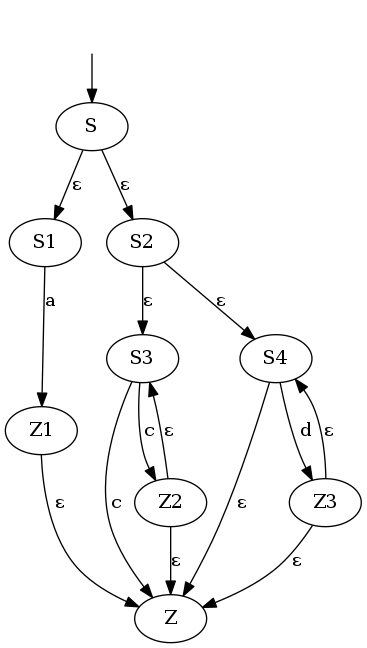
\includegraphics[scale=0.5]{e1.png}

\section{$e2 = a a^{*} b $}
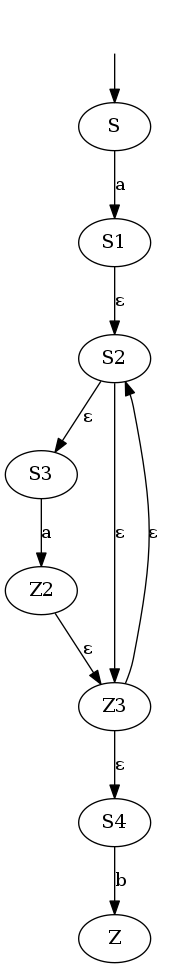
\includegraphics[scale=0.5]{e2.png}
    
\section{$e3 = a + a^{*} b $}
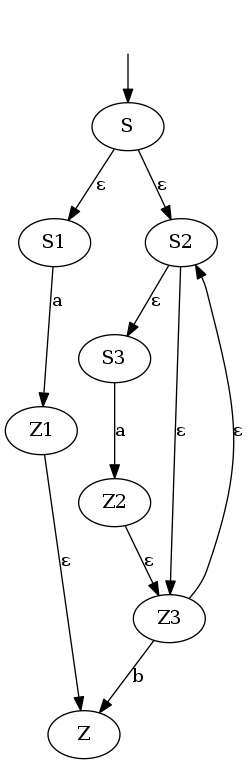
\includegraphics[scale=0.5]{e3.png}

\section{$e4 = a + (a b)^{*} $}
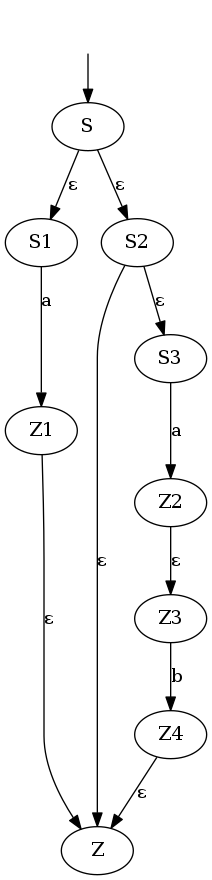
\includegraphics[scale=0.5]{e4.png}

\section{$e5 = c +\ (a + b)^{*} $}
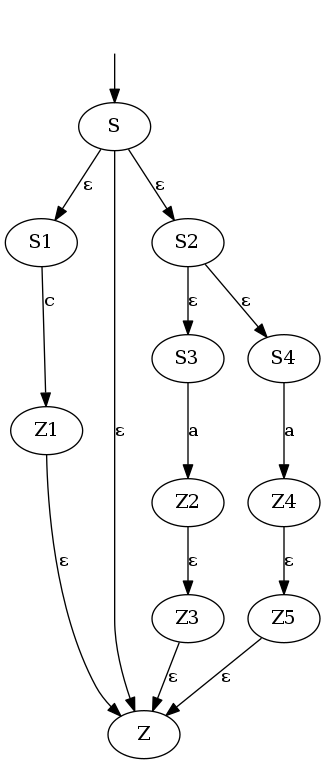
\includegraphics[scale=0.5]{e5.png}



\end{document}
